%----------------------------------------------------------------------------
%----------------------------------------------------------------------------
%				    	SETUP
%----------------------------------------------------------------------------
%----------------------------------------------------------------------------

\documentclass[11pt]{article}

%----------------------------------------------------------------------------
%			  	   PACKAGES
%----------------------------------------------------------------------------

%%%%%%%%%%%%%%%%%%%%%%%
% 	  Packages
%%%%%%%%%%%%%%%%%%%%%%%

%% Fonts and Symbols
%% --------------------------
\usepackage{
			amsmath,			% math operators
			amssymb,			% math symbols
%			amsthm,				% theorem environment
			soul,				% strike through with \st{}
			xcolor,				% color!
%			xfrac,				% fancy fractions
}	

\definecolor{mygreen}{rgb}{0,0.6,0}
\definecolor{mygray}{rgb}{0.5,0.5,0.5}
\definecolor{mymauve}{rgb}{0.58,0,0.82}
\definecolor{darkblue}{rgb}{0,0,0.4}	

%% Graphics
%% --------------------
\usepackage{
			graphicx,			% allows insertion of images
			subfigure,			% allows subfigures (a), (b), etc.
}				
\graphicspath{ {graphics/} }	% (graphicx) relative path to graphics folder				

%% Tables
%% --------------------------
\usepackage{
			booktabs,			% better tables, discourages vertical rulings
			multicol,			% allow multi columns
%			tocloft,			% finer control over TOC; enabled below due to subfigure conflict
}
%\usepackage[subfigure]{tocloft}
%\addtocontents{toc}{\cftpagenumbersoff{subsubsection}} % turn off subsubsection page numbers in ToC

%% Layout Alteration
%% --------------------------
\usepackage{			
%			caption,			% line breaks in captions with \\
%			changepage,			% change margins for PARTS of pages with (adjustwidth)
			fancyhdr,			% see config in LAYOUT AND STYLING
			framed,				% nice boxes; used in Supervisor's Approval
%			fullpage,			% set full page margins
			geometry,			% change the margins for specific PAGES
%			lastpage,			% used with (fancyhdr)
			parskip,			% disable indents
%			pdflscape,			% ???
			rotating,			% sideways figures
}
\geometry{						% specify page size options for (geometry)
			a4paper, 			% paper size
			hmargin=1in,		% horizontal margins
			vmargin=1in,		% vertical margins
}	


%% Units
%% --------------------------
\usepackage{
			siunitx,			% has S (decimal align) column type
}
\sisetup{input-symbols = {()},  % do not treat "(" and ")" in any special way
		group-digits  = false, 	% no grouping of digits
%		 load-configurations = abbreviations,
%		 per-mode = symbol,
}

%% Misc
%% --------------------------
\usepackage{
			enumitem,			% better control of enumerations, descriptions, etc
			listings,			% source code import and display
}

\lstset{ %
	language=verilog,				% the language of the code
	basicstyle=\footnotesize,       % the size of the fonts that are used for the code
	numbers=none,                   % where to put the line-numbers
	numberstyle=\tiny\color{mygray},% the style that is used for the line-numbers
	stepnumber=1,                   % the step between two line-numbers. If it's 1, each line
									% 	will be numbered
	numbersep=5pt,                  % how far the line-numbers are from the code
	backgroundcolor=\color{white},  % choose the background color. You must add \usepackage{color}
	showspaces=false,               % show spaces adding particular underscores
	showstringspaces=false,         % underline spaces within strings
	showtabs=false,                 % show tabs within strings adding particular underscores
	frame=single,	                % box the code [single, none]
	rulecolor=\color{black},        % if not set, the frame-color may be changed on line-breaks
									% 	within not-black text (e.g. commens (green here))
	tabsize=2,                      % sets default tabsize to 2 spaces
	captionpos=b,                   % sets the caption-position to bottom
	breaklines=true,                % sets automatic line breaking
	breakatwhitespace=false,        % sets if automatic breaks should only happen at whitespace
	title=\lstname,                 % show the filename of files included with \lstinputlisting;
									% 	also try caption instead of title
	keywordstyle=[1]\bfseries\color{darkblue},    % keyword style for mnemonics
	keywordstyle=[2]\bfseries\color{violet},	% keyword style for . mnemonics
	commentstyle=\color{mygreen},   % comment style
	stringstyle=\color{mymauve},    % string literal style
	escapeinside={\%*}{*)},         % if you want to add a comment within your code
	morekeywords={*,...}           	% if you want to add more keywords to the set
}

%----------------------------------------------------------------------------
%		     MACROS AND COMMANDS
%----------------------------------------------------------------------------

% Defines a new command for the horizontal lines, change thickness here
\newcommand{\HRule}{\rule{\linewidth}{0.5mm}} 

% override S column type with centered text column
\newcommand{\textcol}[1]{\multicolumn{1}{c}{#1}}


%----------------------------------------------------------------------------
%----------------------------------------------------------------------------
%				   DOCUMENT
%----------------------------------------------------------------------------
%----------------------------------------------------------------------------

\begin{document}

%----------------------------------------------------------------------------
%				    TITLE PAGE
%----------------------------------------------------------------------------

\begin{titlepage}

\center
 
% Header
\textsc{\LARGE University of Victoria}\\[1cm] 	% Name of your university/college
\textsc{\Large CENG 241}\\[0.5cm] 			% Major heading such as course name
\textsc{\large Digital Design I}\\[0.5cm] 		% Minor heading such as course title


% Lab Title
\HRule \\[0.4cm]
{\huge \bfseries Lab 2 - Using Xilinx ISE Tutorial}\\[0.2cm] % Title of your document
\HRule \\[1.5cm]
 
 
%Lab Instructor Details
\begin{minipage}{0.7\textwidth}
\begin{flushleft} 

\large\emph{Instructor:} \\
Dr. Amirali \textsc{Baniasadi} \\
\vspace{12 pt}
\emph{Teaching Assistant:} \\
Grace \textsc{Hui}

\end{flushleft}
\end{minipage}
~
%% No content here, but it keeps the alignment of the instructor/TA
%% box correct.
%% Consider revising.
\begin{minipage}{0.1\textwidth}
\begin{flushright} \large
%Dr. Barbara \textsc{Sawicka} \\
\vspace{12 pt}
%\emph{Teaching Assistant:} \\
%Vahid \textsc{Moradi}
\end{flushright}
\end{minipage}\\[2cm]


% Lab members
\Large Yves \textsc{Senechal}
\large V00213837	\\
\Large Tyler \textsc{Stephen}
\large V00812021	\\
A01 - B03\\[1.5cm] 


% Date
{\large 8 June, 2015}\\ % Date, change the \today to a set date if you want to be precise

% Logo
\begin{figure}[b]	 % put logo at bottom of the page
	\centering
	\includegraphics[scale=0.3]{UVic_logo}
\end{figure}

\end{titlepage}

%----------------------------------------------------------------------------
%				    BODY
%----------------------------------------------------------------------------

\section{Introduction}

The second lab serves as a learning environment for the Xilinx ISE (integrated software environment). This software enables simulation of digital circuits which can facilitate the design and troubleshooting of such circuits. Two digital design entry methods were explored: the schematic method, and the Verilog HDL (hardware description language).  

\section{Results}

The following figures are snapshots obtained during this lab. A half adder is illustrated by the schematic in Figure \ref{fig:schematic}. The functional simulation in Figure \ref{fig:functional_sim} shows the expected output from the circuit based on user-defined input. Outputs $S$ and $C$ are shown for all combinations of binary inputs $X$ and $Y$.

\begin{figure}[htbp]
	\centering
	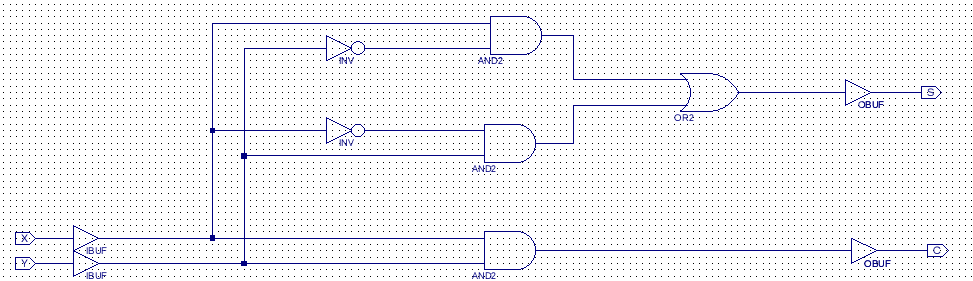
\includegraphics[width=0.95\textwidth, draft=false]{ha_schematic}
	\caption{Complete schematic of a half adder}
	\label{fig:schematic}
\end{figure}

\begin{figure}[htbp]
	\centering
	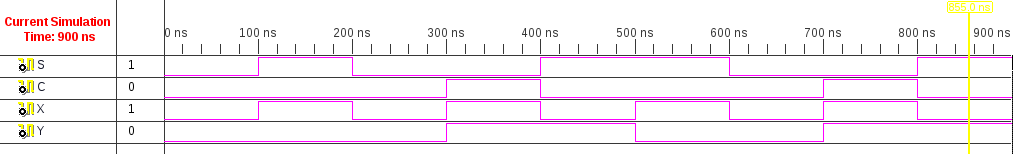
\includegraphics[width=0.95\textwidth, draft=false]{functional_sim}
	\caption{Functional simulation of a half adder}
	\label{fig:functional_sim}
\end{figure}

The Verilog HDL code for a half adder is shown in the code block below, while the post place-and-route timing simulator is shown if Figure \ref{fig:timing}. An FPGA is programmed according to the verilog module, which is used to determine the runtime delay of the half adder. Figure \ref{fig:timing} indicates that both outputs will arrive 8.9 ns after the inputs.

\hspace{1cm}

\lstinputlisting[title=Verilog implementation of a half adder]{ha.v}

\begin{figure}[htbp]
	\centering
	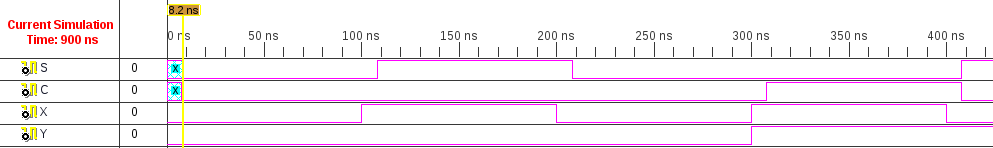
\includegraphics[width=0.95\textwidth, draft=false]{post_place_timing}
	\caption{Post place and route timing indicates a delay of 8.9 ns in the half adder}
	\label{fig:timing}
\end{figure}

\newpage

\section{Discussion}

The digital design entry methods explored were the schematic and Verilog HDL. The Verilog HDL seemed to be more efficient testing logic assuming a proper boolean function was available. This method produces quick results for any size circuit, but could be prone to error due to not being able to visualize the circuit. The schematic method is tedious for anything but few component circuits, but enables visualization which may help troubleshooting.

A functional simulation tests the logic of a circuit with no consideration on circuit timing and delays. Timing simulations, meanwhile, test the functionality of circuits with any routing and logic delay considered to give proper results. Functional simulations can only ensure that the logic of the circuit is correct but give no insight about delays arising from timing problems.



\section{Conclusion}

The two digital design methods explored in this lab offer their individual strengths with their weaknesses. The schematic design is more user friendly, but tedious, while the Verilog HDL is quick and efficient, but could be prone to error. 

\end{document}